%%%%%%%%%%%%%%%%%%%- HXN
\def\sode{13}
\def\tendethi{ĐỀ PHÁT TRIỂN MINH HOẠ 2025}
\begin{dethi}
 {\tendethi}
\end{dethi}
\caulc
\Opensolutionfile{ans}[ans/ans-HXN-\sode-T]
\begin{ex}%Câu 1
 Cho hàm số $ f(x)$ có bảng xét dấu của đạo hàm như sau\\
 \centerline{
 
\begin{tikzpicture}[>=stealth]
 \tkzTabInit[nocadre=false,lgt=1.2,espcl=2.5,deltacl=.5]
 {$x$/.7, $f'(x)$/1}
 {$-\infty$,$-1$,$0$,$3$,$+\infty$}
 \tkzTabLine{ , + , $0$ , - ,$0$,+,$0$,-, }
 \end{tikzpicture}
 }
 Hàm số đã cho nghịch biến trên khoảng nào dưới đây?
 \choice
 {$\left(-1;3\right)$}
 {$\left(-\infty;-1\right)$}
 {\True $\left(-1;0\right)$}
 {$\left(0;+\infty\right)$}
\end{ex}
\begin{ex}%Câu 2
 Chỉ số ô nhiễm không khí (AQI) tại thủ đô Hà Nội trong tháng 6/2024 được thống kê vào lúc 10h30 sáng các ngày trong tháng thể hiện theo bảng số liệu sau:\\
 \centerline{\begin{tblr}{|c|c|c|c|c|c|}
 \hline
 Chỉ số (AQI) & $[130;145)$ & $[145;160)$ & $[160;175)$ & $[175;190)$ & $[190;205)$\\
 \hline
 Số ngày & 8 & 7 & 6 & 7 & 2\\
 \hline
 \end{tblr}}\\
 Tứ phân vị thứ ba của mẫu số liệu trên gần nhất với giá trị nào sau đây?
 \choice
 {$ 175$}
 {$ 176{,}5$}
 {$ 180{,}2$}
 {\True $ 178{,}2$}
\end{ex}
\begin{ex}%Câu 3
 Trong không gian $ Oxyz$, đường thẳng đi qua điểm $ M\left(1;3;-2\right)$ và nhận vectơ $\vec{u}=\left(1;-1;5\right)$ làm vectơ chỉ phương có phương trình tham số là
 \choice
 {$\heva{& x=1+t\\& y=-1+3t\\& z=5-2t}$}
 {$\heva{& x=1+t\\& y=-1+3t\\& z=5+2t}$}
 {\True $\heva{& x=1+t\\& y=3-t\\& z=-2+5t}$}
 {$\heva{& x=1+t\\& y=3+t\\& z=-2+5t}$}
\end{ex}
\begin{ex}%Câu 4
 Khẳng định nào dưới đây là đúng?
\choice
{$\int{x^3\mathrm{\,d}x=x^4}+C$}
{$\int{x^3\mathrm{\,d}x=3x^2}+C$}
{$\int{x^3\mathrm{\,d}x=\dfrac{x^3}{\ln3}}+C$}
{\True $\int{x^3\mathrm{\,d}x=\dfrac{x^4}{4}}+C$}
\end{ex}
\begin{ex}%Câu 5
 Quãng đường đi bộ mỗi ngày (đơn vị: $km$) của Tom trong $20$ ngày gần nhất được thống kê lại ở bảng sau:\\
 \centerline{\begin{tblr}{|c|c|c|c|c|c|}
 \hline
 Quãng đường (km) & $[2,7 ; 3,0)$ & $[3,0 ; 3,3)$ & $[3,3 ; 3,6)$ & $[3,6 ; 3,9)$ & $[3,9 ; 4,2)$\\
 \hline
 Số ngày & 3 & 6 & 5 & 4 & 2\\
 \hline
 \end{tblr}}\\
 Khoảng biến thiên của mẫu số liệu ghép nhóm là
 \choice
 {\True $ 1{,}5$km}
 {$ 0{,}9$km}
 {$ 0{,}6$km}
 {$ 0{,}3$km}
\end{ex}
\begin{ex}%Câu 6
 Tập nghiệm của bất phương trình $\log_{\frac{2}{3}}x>2$ là
 \choice
 {\True $\left(0;\dfrac{4}{9}\right)$}
 {$\left(-\infty;\sqrt[3]{4}\right)$}
 {$\left(\sqrt[3]{4};+\infty\right)$}
 {$\left(-\infty;\dfrac{4}{9}\right)$}
\end{ex}
\begin{ex}%Câu 7
 Trong không gian $ Oxyz$, hình chiếu vuông góc của điểm $ M\left(3;1;-1\right)$ trên trục $ Oy$ có tọa độ là 
 \choice
 {$\left(3;0;-1\right)$}
 {\True $\left(0;1;0\right)$}
 {$\left(3;0;0\right)$}
 {$\left(0;0;-1\right)$}
\end{ex}
\begin{ex}%Câu 8
 Tiệm cận ngang của đồ thị hàm số $ y=\dfrac{2}{x-1}$ là đường thẳng:
 \choice
 {$y=2$}
 {$x=1$}
 {$y=1$}
 {\True $y=0$}
\end{ex}
\begin{ex}%Câu 9
 Cho cấp số cộng $\left(u_n\right)$ có $u_2=2$, $u_5=11$. Công sai $d$ của cấp số cộng là
 \choice
 {1}
 {2}
 {\True 3}
 {4}
\end{ex}
\begin{ex}%Câu 10
\immini
{
 Cho hàm số $ f(x)$ liên tục trên $\left[-1;5\right]$ và có đồ thị trên đoạn $\left[-1;5\right]$ như hình vẽ bên dưới. Tổng giá trị lớn nhất và giá trị nhỏ nhất của hàm số $ f(x)$ trên đoạn $\left[-1;5\right]$ bằng
 \choice
 {$-1$}
 {$ 4$}
 {\True $ 1$}
 {$ 2$}
}
{
 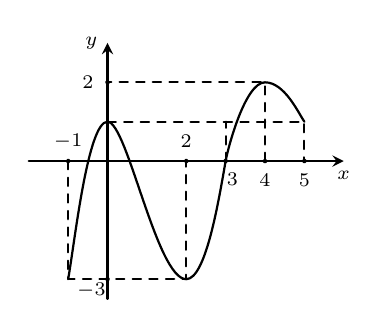
\begin{tikzpicture}[line cap=round, line join=round, scale=0.5,font=\scriptsize,>=stealth,thick]
 \draw[->](-2,0)--(6,0)node[below]{$x$};
 \draw[->](0,-3.5)--(0,3)node[left]{$y$};
 \draw
 (-1,-3)..controls++(80:1) and++(180:0.5)..(0,1)..controls++(0:0.5) and++(180:0.75)..(2,-3)..controls++(0:0.5) and++(-100:1)..(3,0)..controls++(80:0.35) and++(180:0.5)..(4,2)..controls++(0:0.5) and++(125:0.25)..(5,1);
 \foreach \x/\y/\m/\g in{-1/0/-1/90,0/-3/-3/-145,2/0/2/90,3/0/3/-70,4/0/4/-90,5/0/5/-90,0/2/2/180}
 \draw[fill=black](\x,\y)circle(1pt)node[shift={(\g:0.25)}]{$\m$};
 \draw[dashed](-1,0)--(-1,-3)--(0,-3)--(2,-3)--(2,0)(0,1)--(5,1)--(5,0)(3,0)--(3,1)(4,0)--(4,2)--(0,2);
 \end{tikzpicture}
}
\end{ex}
\begin{ex}%Câu 11
 Cho hình hộp $ABCD.A'B'C'D'$. Gọi $O$ là tâm của hình hộp, khẳng định nào dưới đây đúng?
 \choice
 {$\overrightarrow{OA}+\overrightarrow{O{A}'}=\overrightarrow{0}$}
 {\True $\overrightarrow{OA}+\overrightarrow{O{C}'}=\overrightarrow{0}$}
 {$\overrightarrow{OA}+\overrightarrow{OB}=\overrightarrow{0}$}
 {$\overrightarrow{OA}+\overrightarrow{OD}=\overrightarrow{0}$}
\end{ex}
\begin{ex}%Câu 12
 Với $ a,b$ là các tham số thực thì giá trị tích phân $ I=\int\limits_0^b{\left(3x^2-2ax-1\right)\text{d}x}$ bằng
 \choice
 {$b^3-b{a^2}-b$}
 {$b^3+b^2a+b$}
 {\True $b^3-b^2a-b$}
 {$ 3b^2-2ab-1$}
 \end{ex}
\Closesolutionfile{ans}
\cauds
\Opensolutionfile{ans}[ans/ans-HXN-\sode-TF]
\begin{ex}%Câu 13
Nếu đứng trước biển và nhìn ra xa, người ta sẽ thấy một đường giao giữa mặt biển và bầu trời, đó là đường chân trời đối với người quan sát. Ta có thể hình dung rằng nếu người quan sát ở tại đỉnh của một chiếc nón và trái đất được \lq\lq thả\rq\rq vào trong chiếc nón ấy thì đường chân trời là đường \lq\lq chạm\rq\rq giữa trái đất và chiếc nón.\\
\centerline{
 \includegraphics[width=7cm]{img/HXN-13-13}
}
Trong không gian $Oxyz$, giả sử bề mặt trái đất $(S)$ có phương trình $x^2+y^2+z^2=1$ và người quan sát ở vị trí $ B\left(1;1;-1\right)$; $A$ là một vị trí bất kì trên đường chân trời đối với người quan sát ở vị trí $B$.
 \choiceTF
 {\True Khoảng cách từ vị trí $B$ đến tâm của trái đất là $\sqrt{3}$}
 {\True Khoảng cách hai điểm $A$, $B$ là $\sqrt{2}$}
 {Phương trình mặt cầu đường kính $OB$ là $\left(x-\dfrac{1}{2}\right)^2+\left(y-\dfrac{1}{2}\right)^2+\left(z-\dfrac{1}{2}\right)^2=\dfrac{3}{4}$}
 {\True Điểm $A$ luôn thuộc mặt phẳng cố định $ x+y-z-1=0$}
 \loigiai{
     \begin{itemchoice}
         \itemch Tâm của trái đất là điểm $O(0;0;0)$, bán kính $R=1$.\\
         Ta có $OB=\sqrt{(1-0)^2+(1-0)^2+\left(-1-0\right)^2}=\sqrt{3}$.
         \itemch Vì $\triangle OAB$ vuông tại $A$ nên $AB=\sqrt{OB^2-R^2}=\sqrt{3-1}=\sqrt{2}$.
         \itemch Gọi $I$ là trung điểm OB thì $I\left(\dfrac{1}{2};\dfrac{1}{2};-\dfrac{1}{2}\right)$; mặt cầu đường kính OB có tâm $I$,\\
         bán kính $\dfrac{OB}{2}=\dfrac{\sqrt{3}}{2}$ nên có phương trình $\left(S'\right)\colon \left(x-\dfrac{1}{2}\right)^2+\left(y-\dfrac{1}{2}\right)^2+\left(z+\dfrac{1}{2}\right)^2=\dfrac{3}{4}$.
         \itemch Ta thấy $A$ luôn thuộc đường tròn giao tuyến của hai mặt cầu $(S)\,,\left({S'}\right)$.
         Xét hệ phương trình $\heva{& x^2+y^2+z^2=1 \\& \left(x-\dfrac{1}{2}\right)^2+\left(y-\dfrac{1}{2}\right)^2+\left(z+\dfrac{1}{2}\right)^2=\dfrac{3}{4} }  \Leftrightarrow \heva{& x^2+y^2+z^2=1 \\& x^2+y^2+z^2-x-y+z=0 }  \Leftrightarrow \heva{& x^2+y^2+z^2=1 \\& 1-x-y+z=0 } \Leftrightarrow \heva{& x^2+y^2+z^2=1 \\& x+y-z-1=0 }$.\\
         Vậy điểm $A$ luôn thuộc mặt phẳng cố định $x+y-z-1=0$.
     \end{itemchoice}
 }
\end{ex}
\begin{ex}%Câu 14
Một màn ảnh hình chữ nhật cao $1{,}4$ m được đặt ở độ cao $1{,}8$ m so với tầm mắt (tính từ đầu mép dưới của màn hình). Một người đang xem phim có mắt đặt ở vị trí O và quan sát màn ảnh với góc nhìn $\widehat{BOC}$. Với các điểm như trong hình vẽ, đặt $x=OA$, $ x>0$.
\choiceTF
 {\True $\tan\widehat{BOC}=\dfrac{\tan\widehat{AOC}-\tan\widehat{AOB}}{1+\tan\widehat{AOC}\cdot\tan\widehat{AOB}}$}
 {\True $\tan\widehat{AOC}=\dfrac{3{,}2}{x}$, $\tan\widehat{AOB}=\dfrac{1{,}8}{x}$}
 {Nếu góc nhìn màn hình của mắt người là $15^{\circ}$ thì người đó đang ngồi cách bức tường (nơi gắn màn hình) một khoảng gần nhất bằng $3{,}6$ mét (làm tròn đến hàng phần chụ}
 {Người xem muốn nhìn rõ màn ảnh nhất (góc nhìn lớn nhất) thì người đó phải đứng cách mặt phẳng chứa màn ảnh một khoảng $2{,}2$ mét}
 \loigiai{
     \begin{itemchoice}
         \itemch Ta có $\widehat{BOC}=\widehat{AOC}-\widehat{AOB}\Rightarrow \tan\widehat{BOC}=\tan\left(\widehat{AOC}-\widehat{AOB}\right)=\dfrac{\tan\widehat{AOC}-\tan\widehat{AOB}}{1+\tan\widehat{AOC}\cdot \tan\widehat{AOB}}$.
         \itemch Xét lần lượt các tam giác vuông $OAB$, $OAC$ (vuông tại $O$), ta có
         $\tan\widehat{AOC}=\dfrac{AC}{AO}=\dfrac{3{,}2}{x}$, $\tan\widehat{AOB}=\dfrac{AB}{AO}=\dfrac{1{,}8}{x}$.
         \itemch Ta có: $\tan\widehat{BOC}=\dfrac{\dfrac{3{,}2}{x}-\dfrac{1{,}8}{x}}{1+\dfrac{3{,}2}{x}\cdot \dfrac{1{,}8}{x}}=\dfrac{\dfrac{1{,}4}{x}}{\dfrac{x^2+5{,}76}{x^2}}=\dfrac{1{,}4x}{x^2+5{,}76}$.\\
         Khi $\widehat{BOC}=15^{\circ }$ thì $$\tan 15^{\circ}=\dfrac{1{,}4x}{x^2+5{,}76}\Rightarrow \tan 15^{\circ}\cdot x^2-1{,}4x+5{,}76\cdot \tan 15^{\circ}=0\Rightarrow \hoac{& x\approx 3{,}6\,m \\& x\approx 1{,}6\,m.} $$
         Ta chọn $x\approx 1{,}6<3{,}6$.\\
         Vì vậy người xem ngồi cách tường một khoảng gần nhất xấp xỉ $1{,}6$ mét.
         \itemch Ta cần tìm giá trị lớn nhất của hàm $f(x)=\dfrac{1{,}4x}{x^2+5{,}76}$, $x>0$.\\
         Đạo hàm $f'(x)=\dfrac{-1{,}4x^2+8{,}064}{\left(x^2+5{,}76\right)^2}$; $f'(x)=0\Leftrightarrow x^2=5{,}76\Rightarrow x=2{,}4$.\\
         Bảng biến thiên:\\
         
\begin{tikzpicture}[>=stealth]
             \tkzTabInit[nocadre=false,lgt=1.2,espcl=2.5,deltacl=0.5]{$x$/.7 ,$f'(x)$/.7,$f(x)$/2}
             {$-\infty$ , $2{,}4$ , $+\infty$}
             \tkzTabLine{ , + , $0$ , - , }
             \tkzTabVar{-/, +/$\dfrac{7}{24}$ , -/}
         \end{tikzpicture}
         
         Vậy để góc nhìn lớn nhất $\left(\widehat{BOC}_{\max}\right)$ thì $\tan\widehat{BOC}$ đạt giá trị lớn nhất
         $\Leftrightarrow f(x)$ đạt giá trị lớn nhất.\\
         Dựa vào bảng biến thiên, ta thấy $\max\limits_{\left(0;+\infty \right)} f(x)=\dfrac{7}{24}$, khi đó $x=2{,}4$ (mét).
     \end{itemchoice}
 }
\end{ex}
\begin{ex}%Câu 15
Một chậu nước có dạng một khối tròn xoay với thiết diện qua trục của chậu (mặt cắt đi qua hai tâm của hai đường tròn đáy) là hai đường parabol đối xứng nhau qua trục đó. Biết hai đường tròn đáy chậu cùng có bán kính $0{,}5$ m; thiết diện nhỏ nhất vuông góc với trục của chậu có bán kính $0{,}2$ m; chiều cao của chậu nước bằng $1{,}5$ m. Người ta bơm nước vào chậu với tốc độ $5$ lít/phút.\\
Xét hệ trục tọa độ $Oxy$ với gốc $O$ trùng với tâm đường tròn đáy của chậu nước, tia $Ox$ chứa trục của chậu nước (đơn vị trên mỗi trục là mét). Mặt cắt qua trục của chậu nước cho ta hai nhánh parabol như hình vẽ, gọi $ y=f(x)$ là parabol nằm trên trục hoành.
\begin{center}
    \includegraphics[width=5cm]{img/HXN-13-15-a}\includegraphics[height=5cm]{img/HXN-13-15-b}
\end{center}
\choiceTF
 {\True $ f(x)=\dfrac{8}{15}{x^2}-\dfrac{4}{5}x+\dfrac{1}{2}$}
 {\True Sức chứa tối đa của chậu nước bằng $0{,}5$ m$^3$ (làm tròn đến hàng phần chục của mét khối)}
 {\True Sau $1{,}5$ giờ bơm nước (làm tròn đến hàng phần chục của giờ) thì chậu đầy nước}
 {\True Nếu bơm từ đầu như thế thì đến phút thứ $20$, tốc độ dâng lên của nước bằng $0{,}01$ m/phút}
 \loigiai{
     \begin{center}
         \includegraphics[height=5cm]{img/HXN-13-15-LG}
     \end{center}
     \begin{itemchoice}
         \itemch  Parabol $f(x)=ax^2+bx+c$, $\left(a\ne 0\right)$ đi qua các điểm $\left(0;0{,}5\right)$, $\left(1{,}5;0{,}5\right)$, $\left(0{,}75;0{,}2\right)$ nên ta có hệ phương trình $\heva{& c=0{,}5 \\& 1{,}5^2a+1{,}5b+0{,}5=0{,}5 \\& 0{,}75^2a+0{,}75b+0{,}5=0{,}2 } \Rightarrow \heva{& a=\dfrac{8}{15} \\& b=-\dfrac{4}{5} \\& c=\dfrac{1}{2}.} $\\
         Do vậy $f(x)=\dfrac{8}{15}x^2-\dfrac{4}{5}x+\dfrac{1}{2}$.
         \itemch Thiết diện của chậu nước vuông góc với trục $Ox$ tại vị trí có hoành độ $x$ chính là đường tròn có bán kính $r=\dfrac{8}{15}x^2-\dfrac{4}{5}x+\dfrac{1}{2}$ nên có diện tích $S(x)=\pi r^2=\pi \left(\dfrac{8}{15}x^2-\dfrac{4}{5}x+\dfrac{1}{2}\right)^2$.\\
         Thể tích chậu nước là $V_{full}=\int\limits_0^{1{,}5}{S(x)\mathrm{\,d}x}=\int\limits_0^{1{,}5}\pi {\left(\dfrac{8}{15}x^2-\dfrac{4}{5}x+\dfrac{1}{2}\right)^2\mathrm{\,d}x}\approx 0{,}5\,m^3$ (lưu vào A).
         \itemch Đổi đơn vị $5$ lít/phút = $\dfrac{5\colon 1000}{1\colon 60}=\dfrac{3}{10}$ $m^3$/giờ.\\
         Thời gian bơm nước đầy chậu là $\dfrac{V_{full}}{3/10}=\dfrac{49}{100}\pi \approx 1{,}5$ giờ.   [Nhấn máy: A chia $3/10$].
         \itemch Từ câu b) ta thấy hoành độ $x$ $\left(x>0\right)$ cũng chính là chiều cao mực nước trong chậu.\\
         Thể tích chậu nước ứng với chiều cao $x$ là $V=\int\limits_0^x{S(x)\mathrm{\,d}x}$ \tagEX{1}
         Sau $20$ phút bơm nước thì thể tích nước trong chậu là $V_{20}=5\times 20=100$ lít = $0{,}1$ $m^3$/phút.\\
         Xét $V=\int\limits_0^x{S(x)\mathrm{\,d}x}=0{,}1\Rightarrow \int\limits_0^x{\pi \left(\dfrac{8}{15}x^2-\dfrac{4}{5}x+\dfrac{1}{2}\right)^2\mathrm{\,d}x}=0{,}1\Rightarrow x\approx 0{,}164\,m$ (lưu vào B).\\
         Đạo hàm hai vế của $(1)$ theo $t$, ta được\\
         \centerline{$\dfrac{dV}{\mathrm{\,d}t}=S(x)\cdot \dfrac{\mathrm{\,d}x}{\mathrm{\,d}t}\Leftrightarrow \dfrac{dV}{\mathrm{\,d}t}=\pi \left(\dfrac{8}{15}x^2-\dfrac{4}{5}x+\dfrac{1}{2}\right)^2\cdot \dfrac{\mathrm{\,d}x}{\mathrm{\,d}t}$}
         Thay $\dfrac{dV}{\mathrm{\,d}t}=\dfrac{1}{200}\,\,m^3$/phút; $x=B\approx 0{,}164\,m$, ta được $\dfrac{\mathrm{\,d}x}{\mathrm{\,d}t}\approx 0{,}01$ m/phút.
     \end{itemchoice}
 }
\end{ex}
\begin{ex}%Câu 16
\immini
{
    Trong một buổi triển lãm công nghệ quốc tế, công ty A dự định ra mắt sản phẩm mới với sự tham gia của CEO nổi tiếng. Tuy nhiên, có nhiều yếu tố rủi ro có thể khiến sự kiện bị hủy
\begin{itemize}
 \item Nếu lượng khách đăng ký trước vượt 1000 người, sự kiện chắc chắn diễn ra.
 \item Nếu hệ thống máy chủ gặp sự cố (do tấn công mạng hoặc quá tải), công ty không thể xử lý hết số lượng khách đăng ký, khi đó xác suất hủy sự kiện là $60\%$.
 \item Nếu hệ thống hoạt động bình thường, xác suất đủ 1000 đăng ký là $80\%$; nếu không đủ, xác suất hủy sự kiện là $10\%$.
\end{itemize}
}
{
\includegraphics[width=6cm]{img/HXN-13-16}
}
Biết rằng xác suất để sự kiện bị hủy với bất kì lý do gì là $0{,}35$.\\
Gọi các biến cố $A$: \lq\lq Hệ thống gặp sự cố\rq\rq; $B$: \lq\lq Đủ $1000$ đăng ký\rq\rq; $C$: \lq\lq Sự kiện bị hủy\rq\rq.
\choiceTF
 {\True $ P\left(B|A\right)=0$ và $ P\left(\bar{B}|A\right)=1$}
 {\True $ P\left(C|\bar{A}\bar{B}\right)=0{,}1$}
 {Xác suất để hệ thống máy chủ gặp sự cố bằng $0{,}57$ (làm tròn đến hàng phần trăm)}
 {\True Cuối cũng thì những lo lắng cũng đã thành hiện thực, sự kiện quan trọng đã bị hủy, xác suất để hệ thống máy chủ hoạt động bình thường băng $0{,}02$ (làm tròn đến hàng phần trăm)}
 \loigiai{
     \begin{center}
         \includegraphics[height=6cm]{img/HXN-13-16-LG}
     \end{center}
     \begin{itemchoice}
         \itemch Nếu hệ thống gặp sự cố thì số lượng khách hàng đăng ký trước không thể đủ 1000, do đó  $P\left(B|A\right)=0$ và $P\left(\bar{B}|A\right)=1$.
         \itemch Nếu hệ thống máy chủ không gặp sự cố và số lượng đăng ký trước của khách hàng dưới 1000 thì xác suất sự kiện bị hủy bằng $10\%$, do đó $P\left(C|\bar{A}\bar{B}\right)=0{,}1$.
         \itemch Đặt $x=P(A)\in (0;1)$; suy ra $P\left({\bar{A}}\right)=1-x$.\\
         Ta có $P(C)=x\cdot 1\cdot 0{,}6+(1-x)\cdot 0{,}2\cdot 0{,}1=0{,}35\Rightarrow x=\dfrac{33}{58}$ hay $P(A)=\dfrac{33}{58}\approx 0{,}57$.
         \itemch Ta có $P\left(\bar{A}|C\right)=\dfrac{P\left(\bar{A}C\right)}{P(C)}=\dfrac{\left(1-\dfrac{33}{58}\right)\cdot 0{,}2\cdot 0{,}1}{0{,}35}=\dfrac{5}{203}\approx 0{,}02$.
     \end{itemchoice}
 }
\end{ex}
\Closesolutionfile{ans}
\caukq
\Opensolutionfile{ans}[ans/ans-HXN-\sode-SA]
\begin{ex}%Câu 17
\immini
{
     Sau cơn mưa, có 4 cậu bé muốn đi qua một con đê trơn trợt nhưng họ chỉ có hai đôi dép.
 \begin{itemize}
 \item Cậu bé Văn có thể đi qua con đê trong 5 phút.
 \item Cậu bé Võ có thể đi qua con đê trong 9 phút.
 \item Cậu bé Song có thể đi qua con đê trong 13 phút.
 \item Cậu bé Toàn có thể đi qua con đê trong 3 phút.
 \end{itemize}
}
{
    \includegraphics[width=6cm]{img/HXN-13-17}
}
Hỏi thời gian tối thiểu để cả $4$ cậu bé cùng qua được con đê là bao nhiêu phút? Biết rằng mỗi cậu bé muốn đi qua con đê này thì phải mang dép và thời gian để mỗi người đi qua hoặc đi về lại trên con đê là như nhau.
\shortans{31}
\loigiai{
Để tối ưu hóa thời gian qua lại trên con đê thì $2$ cậu bé nhanh nhất (Văn và Toàn) nên đi với nhau, $2$ cậu bé chậm hơn (Võ và Song) nên đi với nhau.\\
Họ phải đi như sau để qua được con đê một cách nhanh nhất:
\begin{itemize}
    \item Văn và Toàn đi cùng nhau $\longrightarrow$ mất 5 phút.
    \item Toàn cầm đôi dép của Văn quay về lại đón bạn $\longrightarrow$ mất 3 phút.
    \item Võ và Song đi cùng nhau $\longrightarrow$ mất 13 phút.
    \item Văn cầm 1 đôi dép quay lại đón bạn $\longrightarrow$ mất 5 phút.
    \item Văn và Toàn đi cùng nhau lần nữa $\longrightarrow$ mất 5 phút.
\end{itemize}
Vậy tổng thời gian ngắn nhất để cả 4 cậu bé qua được con đê là là 31 phút.
}
 \end{ex}
 \begin{ex}%Câu 18
\immini
{
    Một cửa hàng bán lẻ bán được $ 2500$ cái tivi mỗi năm. Để bán được số tivi đó, họ phải đặt hàng từ nhà máy sản xuất tivi nhiều lần trong năm, mỗi lần đặt hàng với số lượng tivi như nhau. Mỗi lần lấy hàng từ nhà máy về thì cửa hàng chỉ trưng bày được một nửa số tivi đó, một nửa số hàng còn lại phải lưu vào kho; chi phí gửi trong kho là $ 10\$$ cho một cái tivi. Chi phí cố định cho mỗi lần đặt hàng là $ 20\$$, ngoài ra cửa hàng phải trả thêm $ 9\$$ cho mỗi tivi. Hỏi mỗi lần đặt hàng trong năm thì cửa hàng cần đặt bao nhiêu tivi để chi phí mà cửa hàng phải trả là nhỏ nhất?
}
{
    \includegraphics[width=6cm]{img/HXN-13-18}
}
\shortans{100}
\loigiai{
Gọi $x$ là số tivi mà cửa hàng đặt mỗi lần $\left(x\in \mathbb{N},\, 1\le x\le 2\,500\right)$.\\
Số tivi lưu vào kho mỗi lần là $\dfrac{x}{2}$; do đó chi phí lưu vào kho là $10\cdot \dfrac{x}{2}=5x$.\\
Số lần đặt hàng trong năm là $\dfrac{2\,500}{x}$ và chi phí đặt hàng là  $\dfrac{2\,500}{x}\left( 20+9x \right)$.\\
Tổng số chi phí mà cửa hàng phải trả là: $\dfrac{2\,500}{x}(20+9x)+5x=5x+\dfrac{50\,000}{x}+22\,500$.\\ 
Áp dụng bất đẳng thức Cauchy ta có  $5x+\dfrac{50\,000}{x}\ge 1\,000$.\\ 
Dấu bằng xảy ra khi $5x=\dfrac{50\,000}{x}\Rightarrow  x=100$.\\  
Vậy mỗi năm cửa hàng cần đặt hàng $\dfrac{2\,500}{100}=25$ lần, mỗi lần $100$ cái.
}
\end{ex}
\begin{ex}%Câu 19
Trong không gian với hệ tọa độ $Oxyz$ cho điểm $A\left(3;2;-1\right)$ và đường thẳng $d\colon \heva{& x=t\\& y=t\\& z=1+t.}$ Tính khoảng cách từ gốc tọa độ đến mặt phẳng $(P)$ biết rằng $(P)$ chứa $d$ sao cho khoảng cách từ $A$ đến $(P)$ là lớn nhất. Làm tròn kết quả đến hàng phần chục.
\shortans{0,8}
\loigiai{
\immini
{
Đường thẳng $d$ qua $M_0(0;0;1)$ có VTCP $\vec{u}=(1;1;1)$.\\
Gọi $H$, $K$ lần lượt là hình chiếu của $A$ lên $(P)$ và $d$ (khi đó $AK$ cố định). Ta có:
$d\left(A,(P)\right)=AH\le AK$.\\
Đẳng thức xảy ra khi và chỉ khi $H\equiv K$.\\
Do đó $d\left(A,(P)\right)_{\max }=AK$.\\
Khi đó $(P)$ đi $M_0(0;0;1)$ nhận $\vec{AK}$ làm vectơ pháp tuyến.
}
{
    \includegraphics[width=6cm]{img/HXN-13-19-LG}
}
Gọi $K\left(t;t;1+t\right)\in d \Rightarrow \vec{AK}=\left(t-3;t-2;t+2\right)$.\\
Ta có $\vec{AK}\perp \vec{u}\Leftrightarrow \vec{AK}\cdot \vec{u}=0 \Leftrightarrow 1\cdot (t-3)+1\cdot (t-2)+1\cdot (t+2)=0\Leftrightarrow t=1$.\\
Suy ra $\vec{AK}=(-2;-1;3)$.\\
Vậy phương trình $(P)\colon -2(x-0)-1\cdot (y-0)+3\cdot (z-1)=0 \Leftrightarrow 2x+y-3z+3=0$.\\
Khi đó: $d\left(O,(P)\right)=\dfrac{3}{\sqrt{4+1+9}}=\dfrac{3\sqrt{14}}{14}\approx 0{,}8$.
}
\end{ex}
\begin{ex}%Câu 20
\immini
{
    Hộp I có 5 quả bóng đỏ và 3 quả bóng trắng, hộp II có 2 quả bóng đỏ và 2 quả bóng trắng, hộp III có 3 quả bóng đỏ và 1 quả bóng trắng. Người ta thực hiện các hành động sau một cách ngẫu nhiên:
}
{
    \includegraphics[width=6cm]{img/HXN-13-20}
}
\begin{itemize}
    \item Lấy 1 quả bóng từ hộp I bỏ sang hộp II.
    \item Lấy 1 quả bóng từ hộp III bỏ sang hộp II.
    \item Lấy ra mỗi hộp 1 quả bóng thì nhận thấy đó là 3 quả bóng trắng.
\end{itemize}
Tính xác suất để cả 3 quả bóng được lấy từ ba hộp vốn là của hộp I và hộp III (ban đầu).\\
Kết quả được làm tròn đến hàng phần trăm.
\shortans{0,13}
\loigiai{
    \begin{center}
        \includegraphics[width=10cm]{img/HXN-13-20-LG}
    \end{center}
    Gọi A là biến cố: \lq\lq Lấy được $3$ quả bóng trắng từ ba hộp\rq\rq và B là biến cố: \lq\lq Cả $3$ quả bóng được lấy từ ba hộp vốn là của hộp I và hộp II\rq\rq.\\
    Để biến cố A xảy ra thì quả bóng chuyển từ hộp III qua hộp II phải là bóng đỏ (vì khi đó hộp III còn 1 quả bóng trắng để lấy ra).\\
    Ta tính xác suất của A trong hai trường hợp quả bóng được chuyển từ hộp I sang hộp II là đỏ hoặc trắng.\\
    Ta có $P(A)=\dfrac{3}{8}\cdot \dfrac{2}{7}\cdot \dfrac{3}{4}\cdot \dfrac{1}{3}\cdot \dfrac{1}{2}+\dfrac{5}{8}\cdot \dfrac{3}{7}\cdot \dfrac{3}{4}\cdot \dfrac{1}{3}\cdot \dfrac{2}{6}=\dfrac{1}{28}$.\\
    Do đó: $P\left(B|A\right)=\dfrac{P(BA)}{P(A)}=\dfrac{\dfrac{3}{8}\cdot \dfrac{2}{7}\cdot \dfrac{3}{4}\cdot \dfrac{1}{3}\cdot \dfrac{1}{6}}{\dfrac{1}{28}}=\dfrac{1}{8}\approx 0{,}13$.
}
\end{ex}
\begin{ex}%Câu 21
\immini
{
    Trong phòng thí nghiệm vật lý, một chất điểm đặt ở vị trí $A$ của hình lập phương được tác động bởi ba lực $\overrightarrow{F_1}$, $\overrightarrow{F_2}$, $\overrightarrow{F_3}$ dọc theo hai cạnh và đường chéo lớn của hình lập phương đó (tham khảo hình vẽ). Biết độ lớn các lực trên hai cạnh bằng $2$ N và $3$ N, độ lớn lực dọc theo đường chéo lớn lập phương bằng $4$ N. Tính độ lớn hợp lực $\left|\overrightarrow{F_1}+\overrightarrow{F_2}+\overrightarrow{F_3}\right|$ theo đơn vị N, làm tròn đến hàng phần trăm.
\shortans{7,22}
}
{
    \includegraphics[width=6cm]{img/HXN-13-21}
}
\loigiai{
Xét $\left(\vec{F_1},\vec{F_2}\right)=90^\circ$; $\left(\vec{F_1},\vec{F_3}\right)=\widehat{BAC'}\Rightarrow \tan \left(\vec{F_1},\vec{F_3}\right)=\tan \widehat{BAC'}=\dfrac{BC'}{AB}=\dfrac{a\sqrt{2}}{a}=\sqrt{2}$\\
$ \Rightarrow \cos \widehat{BAC'}=\sqrt{\dfrac{1}{1+\tan ^2\alpha }}=\dfrac{\sqrt{3}}{3}$; $\left(\vec{F_2},\vec{F_3}\right)=\widehat{DAC'}=\widehat{BAC'}\Rightarrow \cos \left(\vec{F_2},\vec{F_3}\right)=\dfrac{\sqrt{3}}{3}$.\\
Ta có $\left| \vec{F_1}+\vec{F_2}+\vec{F_3} \right|^2=\left| \vec{F_1} \right|^2+\left| \vec{F_2} \right|^2+\left| \vec{F_3} \right|^2+2\vec{F_1}\cdot \vec{F_2}+2\vec{F_1}\cdot \vec{F_3}+2\vec{F_2}\cdot \vec{F_3}$; trong đó:
\begin{itemize}
    \item $2\vec{F_1}\cdot \vec{F_2}=0$ vì $\vec{F_1}\perp \vec{F_2}$.
    \item $2\vec{F_1}\cdot \vec{F_3}=2\left| \vec{F_1} \right|\cdot \left| \vec{F_3} \right|\cos \left(\vec{F_1},\vec{F_3}\right)=2.2\cdot 4\cdot \dfrac{\sqrt{3}}{3}=\dfrac{16\sqrt{3}}{3}$.
    \item $2\vec{F_2}\cdot \vec{F_3}=2\left| \vec{F_2} \right|\cdot \left| \vec{F_3} \right|\cos \left(\vec{F_2},\vec{F_3}\right)=2.3\cdot 4\cdot \dfrac{\sqrt{3}}{3}=8\sqrt{3}$.
\end{itemize}
Do vậy $\left| \vec{F_1}+\vec{F_2}+\vec{F_3} \right|^2=4+9+16+\dfrac{16\sqrt{3}}{3}+8\sqrt{3}=\dfrac{87+40\sqrt{3}}{3}$\\
$\Rightarrow \left| \vec{F_1}+\vec{F_2}+\vec{F_3} \right|=\sqrt{\dfrac{87+40\sqrt{3}}{3}}\approx 7{,}22$N.
}
\end{ex}
\begin{ex}%Câu 22
\immini
{
    Một chiếc trống có đường sinh là các nửa elip tương ứng với độ dài trục lớn $80$ cm, còn độ dài trục bé bằng $60$ cm ; hai đáy trống là các hình tròn có bán kính $60$ cm. Hỏi thể tích của chiếc trống là bao nhiêu dm$^3$ (làm tròn đến hàng đơn vị).
\shortans{345}
}
{
    \includegraphics[width=6cm]{img/HXN-13-22}
}
\loigiai{
    \begin{center}
        \includegraphics[width=6cm]{img/HXN-13-22-LG}
    \end{center}
Đặt hệ trục tọa độ $Oxy$ như hình vẽ, đơn vị trên mỗi trục là dm.
Giả sử elip $(E)$ có độ dài trục lớn $2a=8\Rightarrow a=4$; độ dài trục bé $2b=6\Rightarrow b=3$.\\
Do đó phương trìn $(E)\colon \dfrac{x^2}{16}+\dfrac{y^2}{9}=1\Rightarrow y^2=9\left(1-\dfrac{x^2}{16}\right)$.\\
Ta chọn nửa elip $(E)$ nằm dưới trục hoành là $y=-3\sqrt{1-\dfrac{x^2}{16}}$ $\left(y\le 0\right)$.\\
Để có được hàm số $y=f(x)$ (đường sinh của chiếc trống), ta cần tịnh tiến đồ thị hàm số $y=-3\sqrt{1-\dfrac{x^2}{16}}$ lên trên 6 đơn vị; khi đó $f(x)=6-3\sqrt{1-\dfrac{x^2}{16}}$.\\
Thể tích cái trống là $V=\pi \displaystyle\int\limits_{-4}^4{\left(f(x)\right)^2\mathrm{\,d}x}=\pi \displaystyle\int\limits_{-4}^4{\left(6-3\sqrt{1-\dfrac{x^2}{16}}\right)^2\mathrm{\,d}x}\approx  345\,dm^3$.
}
\end{ex}
\Closesolutionfile{ans}
\inputansbox{6,4,3}{ans/ans-HXN-\sode-T,ans/ans-HXN-\sode-TF,ans/ans-HXN-\sode-SA}